\documentclass{article}

\usepackage[solutions]{xrcise}

\begin{document}
\sheet{Suchen: Bäume \& Hashing}
\begin{exercise}{Rot-Schwarz-Bäume}
  Führen Sie die folgenden Operationen (einfügen bzw. löschen von Schlüsseln) mit einem initial leeren Rot-Schwarz-Baum aus. Geben Sie den Baum nach jedem Einfügen bzw. Löschen sowie nach jeder Rotation bzw. Umfärbung an.
  \begin{align*}\texttt{Insert(40), Insert(48), Insert(68), Insert(55), Insert(39), Delete(40), Delete(48)}\end{align*}

  \begin{solution}
    \begin{figure}[ht]
  \captionsetup[subfloat]{labelformat=empty}

  \begin{tabular}{ccccc}

    \subfloat[\texttt{Insert(40)}]{
      \begin{tikzpicture}
        \node [circle] (z){$40$}
        child[missing] {}
        child[missing] {};
      \end{tikzpicture}
    } &

    \subfloat[fix II.]{
      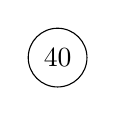
\begin{tikzpicture}
        \node [circle,draw] (z){$40$}
        child[missing] {}
        child[missing] {};
      \end{tikzpicture}
    } &

    \subfloat[\texttt{Insert(48)}]{
      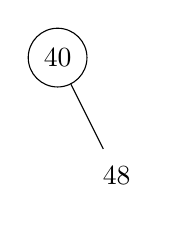
\begin{tikzpicture}
        \node [circle,draw] (z){$40$}
        child[missing] {}
        child {
            node [circle] (a) {48}
            child[missing] {}
            child[missing] {}
          };
      \end{tikzpicture}
    } &

    \subfloat[\texttt{Insert(68)}]{
      \begin{tikzpicture}
        \node [circle,draw] (z){$40$}
        child[missing] {}
        child {
            node [circle] (a) {48}
            child[missing] {}
            child {
                node [circle] (b) {68}
                child[missing] {}
                child[missing] {}
              }
          };
      \end{tikzpicture}
    } &

    \subfloat[fix IV.6]{
      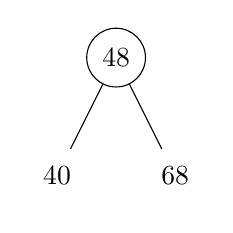
\begin{tikzpicture}
        \node [circle,draw] (z){$48$}
        child {
            node [circle] (a) {40}
            child[missing] {}
            child[missing] {}
          }
        child {
            node [circle] (b) {68}
            child[missing] {}
            child[missing] {}
          };
      \end{tikzpicture}
    }   \\

    \subfloat[\texttt{Insert(55)}]{
      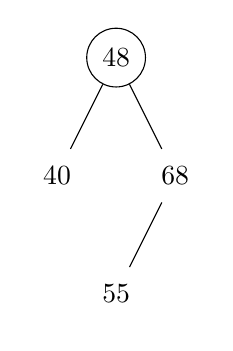
\begin{tikzpicture}
        \node [circle,draw] (z){$48$}
        child {
            node [circle] (a) {40}
            child[missing] {}
            child[missing] {}
          }
        child {
            node [circle] (b) {68}
            child {
                node [circle] (c) {55}
                child[missing] {}
                child[missing] {}
              }
            child[missing] {}
          };
      \end{tikzpicture}
    } &

    \subfloat[fix IV.4]{
      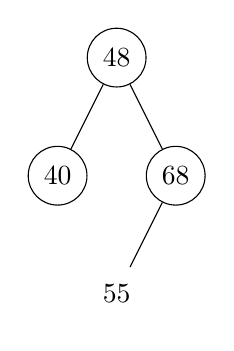
\begin{tikzpicture}
        \node [circle,draw] (z){$48$}
        child {
            node [circle,draw] (a) {40}
            child[missing] {}
            child[missing] {}
          }
        child {
            node [circle,draw] (b) {68}
            child {
                node [circle] (c) {55}
                child[missing] {}
                child[missing] {}
              }
            child[missing] {}
          };
      \end{tikzpicture}
    } &

    \subfloat[\texttt{Insert(39)}]{
      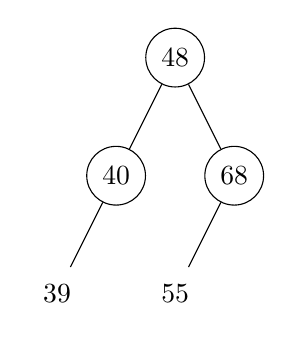
\begin{tikzpicture}
        \node [circle,draw] (z){$48$}
        child {
            node [circle,draw] (a) {40}
            child {
                node [circle] (c) {39}
                child[missing] {}
                child[missing] {}
              }
            child[missing] {}
          }
        child {
            node [circle,draw] (b) {68}
            child {
                node [circle] (d) {55}
                child[missing] {}
                child[missing] {}
              }
            child[missing] {}
          };
      \end{tikzpicture}
    } &

    \subfloat[\texttt{Delete(40)}]{
      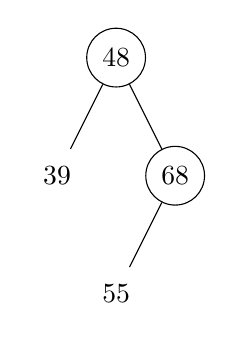
\begin{tikzpicture}
        \node [circle,draw] (z){$48$}
        child {
            node [circle] (a) {39}
            child[missing] {}
            child[missing] {}
          }
        child {
            node [circle,draw] (b) {68}
            child {
                node [circle] (d) {55}
                child[missing] {}
                child[missing] {}
              }
            child[missing] {}
          };
      \end{tikzpicture}
    } &

    \subfloat[fix IV.3]{
      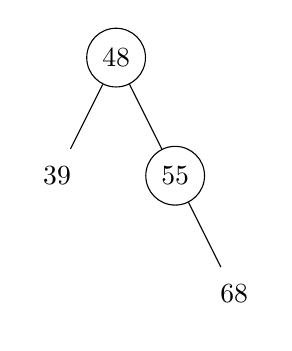
\begin{tikzpicture}
        \node [circle,draw] (z){$48$}
        child {
            node [circle] (a) {39}
            child[missing] {}
            child[missing] {}
          }
        child {
            node [circle,draw] (b) {55}
            child[missing] {}
            child {
                node [circle] (c) {68}
                child[missing] {}
                child[missing] {}
              }
          };
      \end{tikzpicture}
    }   \\

    \subfloat[fix IV.4]{
      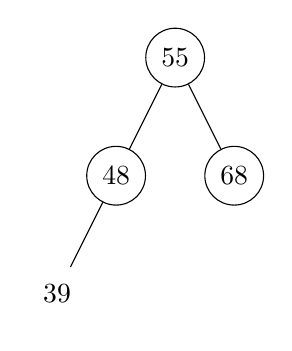
\begin{tikzpicture}
        \node [circle,draw] (z){$55$}
        child {
            node [circle,draw] (a) {48}
            child {
                node [circle] (b) {39}
                child[missing] {}
                child[missing] {}
              }
            child[missing] {}
          }
        child {
            node [circle,draw] (c) {68}
            child[missing] {}
            child[missing] {}
          };
      \end{tikzpicture}
    } &

    \subfloat[\texttt{Delete(48)}]{
      \centering
      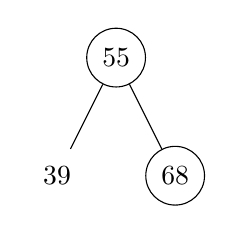
\begin{tikzpicture}
        \node [circle,draw] (z){$55$}
        child {
            node [circle] (a) {39}
            child[missing] {}
            child[missing] {}
          }
        child {
            node [circle,draw] (b) {68}
            child[missing] {}
            child[missing] {}
          };
      \end{tikzpicture}
    } &

    \subfloat[fix IV.2]{
      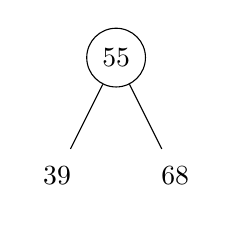
\begin{tikzpicture}
        \node [circle,draw] (z){$55$}
        child {
            node [circle] (a) {39}
            child[missing] {}
            child[missing] {}
          }
        child {
            node [circle] (b) {68}
            child[missing] {}
            child[missing] {}
          };
      \end{tikzpicture}
    }
  \end{tabular}

  \caption{Rot-Schwarz-Baum nach Einfüge- und Löschoperationen}\label{fig:rbinsdel}
\end{figure}
  \end{solution}
\end{exercise}

\begin{exercise}{Hashtabellen}
  Konstruieren Sie die Hashtabelle der Größe $m = 23$, die durch Einfügen der Elemente
  \begin{align*}47, 17, 24, 70, 22, 01, 40, 45, 36, 59\end{align*}
  mit der nachfolgenden Methode entsteht:
  \begin{enumerate}
    \item Divisionsmethode,
    \item Multiplikationsmethode mit $c = 1/2$ und
    \item erweiterter Divisionsmethode mit $a = 5$ und $b = 3$
  \end{enumerate}

  \begin{solution}
    \begin{enumerate}
      \item $[1: 47,24,70,01|13: 36,59|17: 17,40]$ mit $h(k) = k \mod m$
      \item $[0: 24,70,22,40,36|12:47,17,01,45,59]$ mit $h(k) = \lfloor m(kA \mod 1) \rfloor$
      \item $[8: 47,24,70,1|19: 17,40|21: 22,45|22: 36,59]$ mit $h(k) = (ak+b) \mod m$
    \end{enumerate}
  \end{solution}
\end{exercise}

\begin{exercise}{Suchbäume}
  Im Folgenden betrachten wir Zahlen $n = 2^k - 1$ mit $k \in \mathbb{N}_{>0}$.
  \begin{enumerate}
    \item In welcher Reihenfolge sollten die Zahlen in $[1\dots n]$ in einen initial leeren Suchbaum eingefügt werden, damit dieser möglichst balanciert/niedrig ist? Begründen Sie Ihre Antwort kurz.
    \item\label{suchbäume:2} Geben Sie Pseudocode für ein Verfahren mit $\bigO(n)$ Laufzeit an, dass einen entsprechenden Suchbaum erzeugt. Geben Sie eine kurze Begründung an, weshalb ihr Verfahren korrekt ist und die entsprechende Laufzeit erreicht.
    \item Entwerfen Sie einen Algorithmus, der in linearer Laufzeit einen beliebigen Suchbaum mit $n$ Einträgen in einen balancierten Suchbaum umwandelt. Begründen Sie kurz Laufzeit und Korrektheit des Verfahrens. Pseudocode muss nicht angegeben werden.
  \end{enumerate}

  \begin{solution}
    \begin{enumerate}
      \item Die Zahlen sollten rekursiv aus der Mitte heraus eingefügt (möglichst immer den Median). Dies garantiert einen balancierten Baum, da die Anzahl der Knoten in den Teilbäumen immer gleichmäßig aufgeteilt wird.
      \item Ein rekursiver Ansatz:\par
            \begin{algorithm}[H]
  \caption{\texttt{INSERT-SORTED(x, A)}}\label{alg:insertsorted}

  \KwData{Wurzel eines (leeren) Suchbaums $x$, sortierter Array $A$}
  \KwResult{balancierter Suchbaum T}
  \BlankLine

  $median \gets \lfloor A.size/2 \rfloor$\;

  \lIf{$x$ has no children}{\textbf{continue}}
  \lElseIf{$x.key < A[median]$}{$x\gets x.left$}
  \lElse{$x\gets x.right$}

  $x.key = A[median]$\;
  \texttt{INSERT-SORTED($x, A[\text{:median-1}]$)}\;
  \texttt{INSERT-SORTED($x, A[\text{median+1:}]$)}
\end{algorithm}
            Die Laufzeit ist $\bigO(n)$, da jeder Knoten genau einmal besucht wird.
      \item Hierfür lässt sich der Baum in einen sortierten Array umwandeln und dann kann einfach der Algorithmus aus \ref{suchbäume:2} angewandt werden. Die Laufzeit ist $\bigO(n)$, da ein Suchbaum in $\bigO(n)$ in ein sortiertes Array konvertiert wird und der Algorithmus aus \ref{suchbäume:2} ebenfalls in $\bigO(n)$ arbeitet.
    \end{enumerate}
  \end{solution}
\end{exercise}

\begin{exercise}{Hashing}
  Wir betrachten Hashing mit offener Adressierung und quadratischer Sondierung, also eine Hashfunktion der Form $h(k, i) = (h_0(k) + c_1i + c_2i^2) \mod m$. Es seien $h_0(x) = x \mod 13$, sowie $c_1 = c_2 = 1/2$.
  \begin{enumerate}
    \item Fügen Sie die Elemente $938, 1243, 10026, 71, 831, 555, 142, 768, 301, 176, 9347, 32418$ und $360$ in der angegebenen Reihenfolge in eine Hashtabelle der Größe $m = 13$ ein. Stellen Sie das Verfahren graphisch dar. Dabei sollte klar werden wo Kollisionen auftreten und wie diese aufgelöst werden.
    \item Was passiert, wenn als letzte Zahl anstatt der $360$ eine $359$ eingefügt wird?
  \end{enumerate}

  \begin{solution}
    \begin{enumerate}
      \item Die Hashtabelle sieht wie folgt aus:\par
            \begin{table*}[ht]
  \centering
  \begin{tabular}{|c|c|c|c|c| c|c|c|c|c| c|c|c|}
    0   & 1   & 2   & 3     & 4   & 5   & 6  & 7   & 8    & 9   & 10   & 11    & 12  \\
    142 & 768 & 938 & 10026 & 360 & 301 & 71 & 176 & 1243 & 555 & 9347 & 32418 & 831 \\
    i=1 &     &     &       & i=6 & i=2 &    &     &      &     & i=4  & i=5   &     \\
  \end{tabular}

  \caption{Hashtabelle}\label{tbl:hashtable}
\end{table*}
      \item Die quadratische Sondierung schlägt fehl und terminiert nie für 359.
    \end{enumerate}
  \end{solution}

\end{exercise}
\begin{exercise}{Bäume als Graphen}
  Es sei $G = (V, E)$ ein ungerichteter Graph. Zeigen Sie:
  \begin{enumerate}
    \item Es gilt $\sum_{v \in V} \text{deg}(v) = 2|E|$.
    \item Wenn $G$ zusammenhängend (verbunden) ist, dann gilt $|E| \geq |V| - 1$.
    \item Wenn $G$ azyklisch ist, dann gilt $|E| \leq |V| - 1$.
    \item Wenn $G$ ein Baum ist, dann gilt $|E| = |V| - 1$.
    \item Bäume sind kantenmaximal kreisfrei und kantenminimal zusammenhängend. Wird also eine Kante hinzugefügt bzw. entfernt, so ist der entsprechende Graph nicht mehr kreisfrei bzw. zusammenhängend.
  \end{enumerate}

  \begin{solution}
    \begin{enumerate}
      \item Eine Kante verbindet immer zwei Vertices, entsprechen die kumulierten Grade genau der doppelten Anzahl an Kanten.
      \item Ein zusammenhängender Graph hat mindestens $|V| - 1$ Kanten, da jeder Knoten mit mindestens einem anderen Knoten verbunden sein muss.
      \item Ein azyklischer Graph hat höchstens $|V| - 1$ Kanten, da Knoten nur einmal (auch indirekt) miteinander verbunden sein können.
      \item Ein Baum ist ein zusammenhängender azyklischer Graph, also lässt sich die Aussage aus den vorherigen beiden Punkten ableiten.
      \item Es kann keine Kante hinzugefügt werden, ohne einen Kreis zu erzeugen, da bereits alle Knoten (indirekt) verbunden sind. Falls eine Kante entfernt wird, wäre ein Knoten nicht mehr verbunden.
    \end{enumerate}
  \end{solution}
\end{exercise}

\begin{exercise}{Rot-Schwarz-Bäume}
  Gegeben seien zwei Rot-Schwarz-Bäume $B_1$ und $B_2$ und ein Element $x \in \mathbb{Z}$, sodass für alle $x_1 \in B_1$ und $x_2 \in B_2$ gilt: $x_1.\text{key} \leq x \leq x_2.\text{key}$.
  \begin{enumerate}
    \item Beschreiben Sie einen Algorithmus, welcher aus der Vereinigung $B = B_1 \cup \{x\} \cup B_2$ einen neuen Rot-Schwarz-Baum in $\bigO(\log n)$ Zeit berechnet, wobei $n$ die Gesamtanzahl aller Knoten in $B_1$ und $B_2$ ist.
    \item Begründen Sie, warum Ihr Algorithmus die Laufzeitschranke einhält.
  \end{enumerate}

  \begin{solution}
    \begin{enumerate}
      \item Ein möglicher Algorithmus würde von $x$ als neuer Wurzel $B_1$ als linken Teilbaum und $B_2$ als rechten Teilbaum anhängen. Falls die Schwarzhöhe des linken Teilbaums überwiegt, würde eine Rotation nach rechts durchgeführt und umgekehrt.
            \hint{Vereinfachend wird angenommen, dass $x$ nicht in $B_1$ enthalten ist.}
      \item Die Laufzeit ist $\bigO(\log n)$, da die Höhe des Baums $\log n$ ist und somit maximal so viele Rotationen durchgeführt werden müssten (Wenn alle Knoten in einem Teilbaum sind).
    \end{enumerate}
  \end{solution}
\end{exercise}
\end{document}